\begin{frame}
    \centering
    \Large\textbf{Unified Control-Theoretic Training}
\end{frame}

\begin{frame}{\small \textbf{Step back from direct-shooting methods} and consider a \textbf{control-theoretic} training,}
    \footnotesize
        \begin{figure}
            \centering
            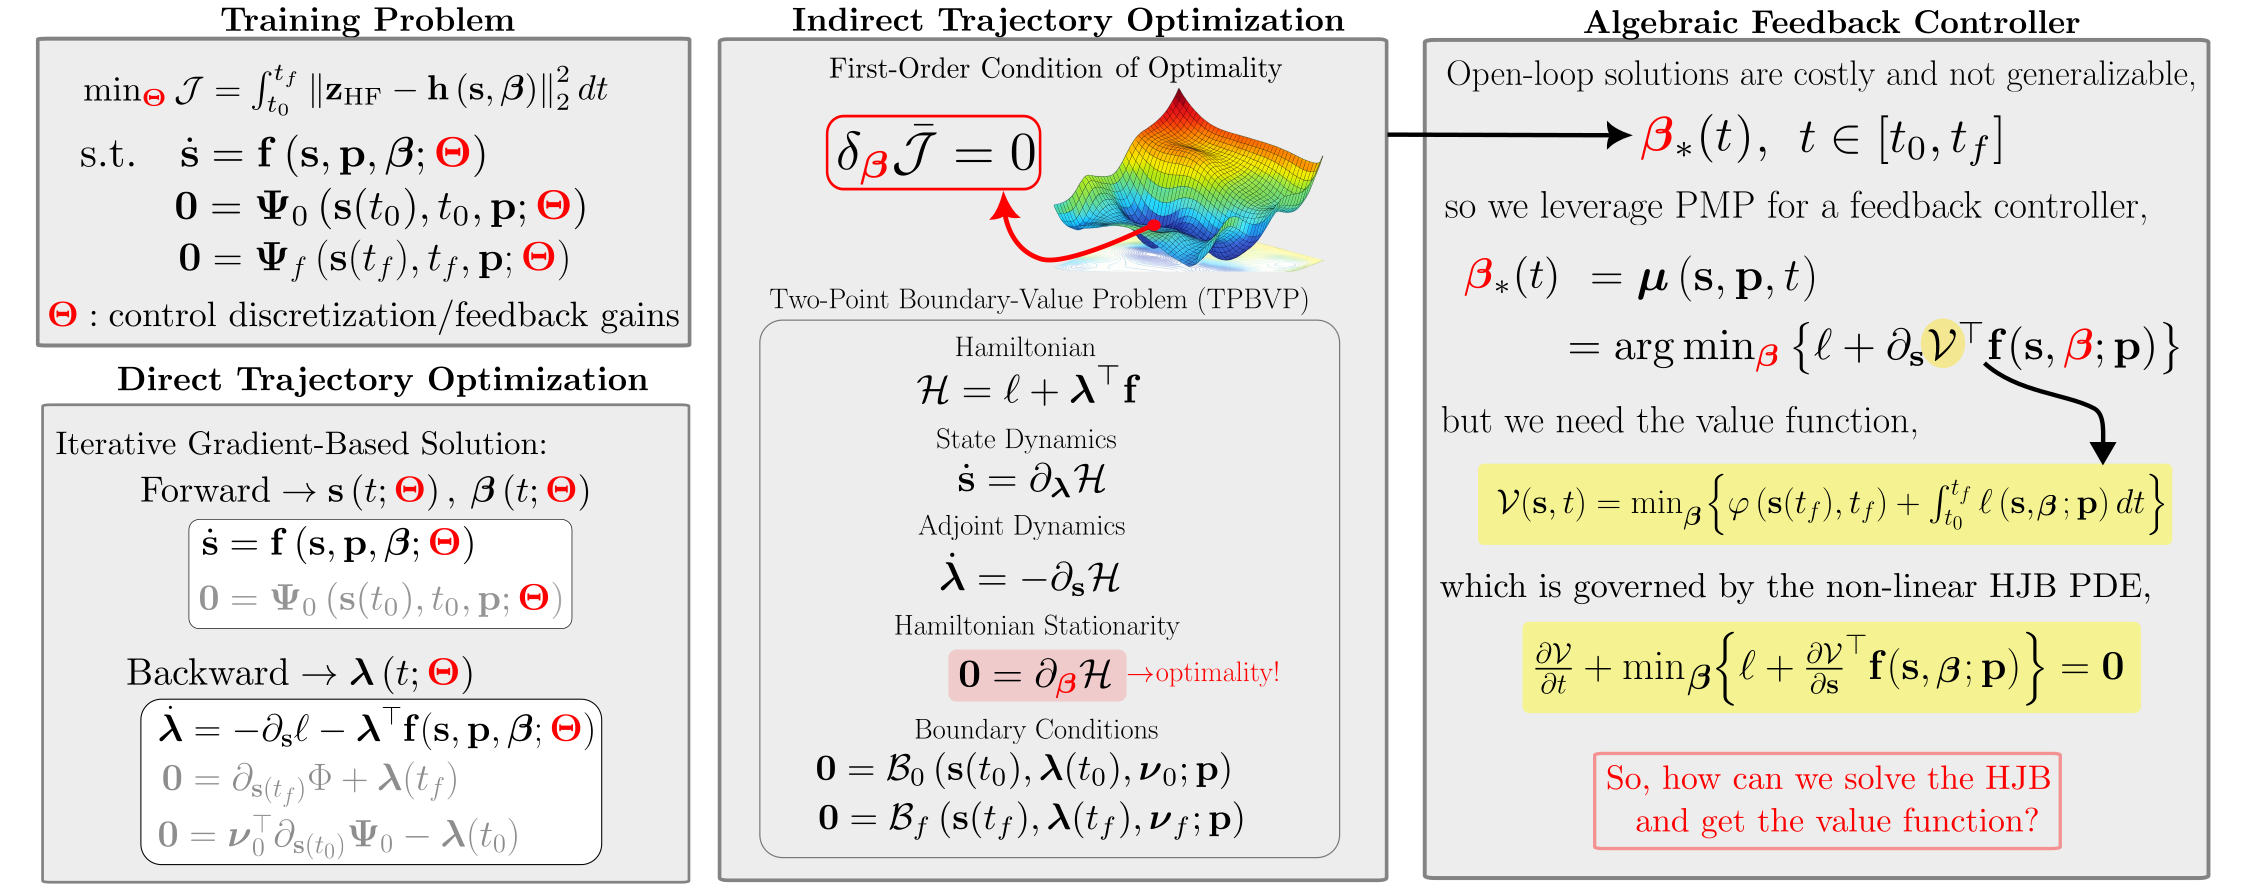
\includegraphics[width=0.95\textwidth]{../figs/ct/ct_overview_19.png}
        \end{figure}
    \begin{center}
        {\tiny
        $\vs$: state, $\Phi$: penalized terminal constraint, $\vbeta$: control action, $\cB_0,\cB_f$: boundary conditions, $\vnu$: Lagrange multipliers, $\vf$: non-linear dynamics, $\bar{\cJ}$: augmented cost functional, PMP: Pontryagin's Minimum Principle, HJB: Hamilton-Jacobi-Bellman}
    \end{center}
\end{frame}

\begin{frame}
    \centering
    \Large\textbf{Addressing the Impossible Trinity of Optimal Control}
\end{frame}

\begin{frame}{\small How can we leverage the \textbf{control-theoretic} training for optimal closed-loop control?}
    \begin{center}
        {\small\textbf{Let us consider the following example}:}\\
        {\small On-board optimal closed-loop control of a hypersonic vehicle}
    \end{center}
    \vspace*{-0.2in}
    \begin{figure}
        \centering
        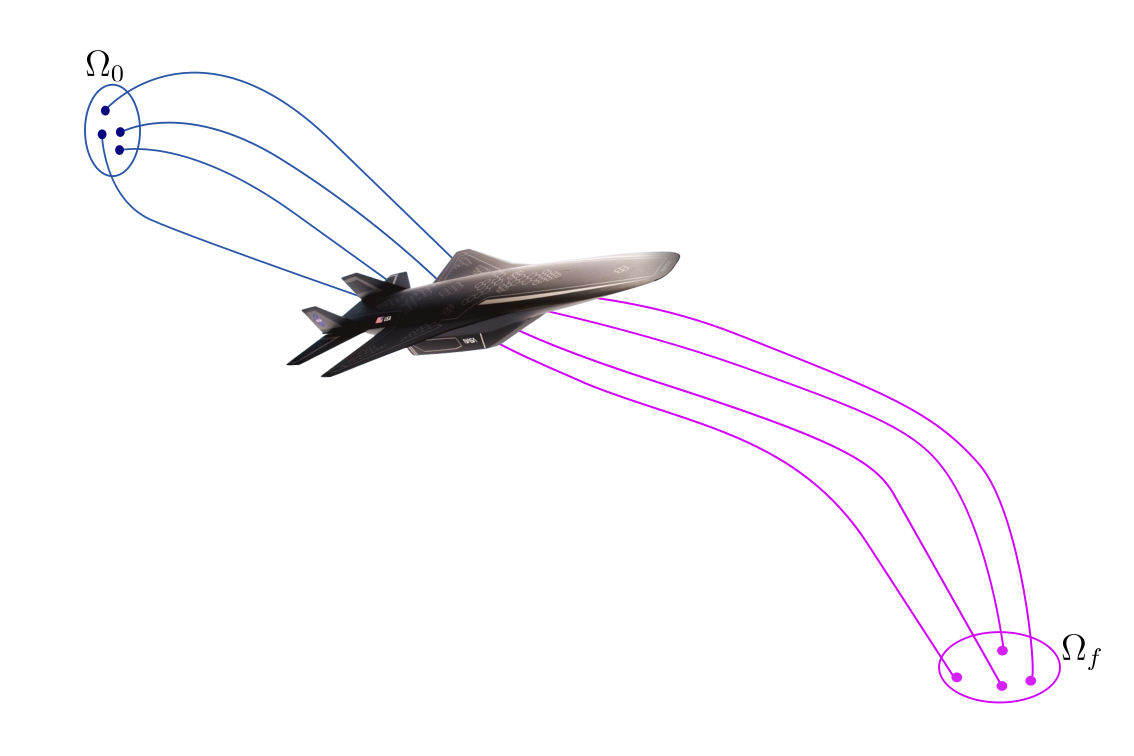
\includegraphics[width=0.6\textwidth]{../figs/introduction/motivating_example_1.png}
    \end{figure}
\end{frame}

\begin{frame}{\small We want \textbf{accuracy, efficient, and generalizable} solutions to \textbf{non-linear OCPs},}
    \footnotesize
    \begin{columns}
        \begin{column}{0.7\textwidth}
            \begin{figure}
                \centering
                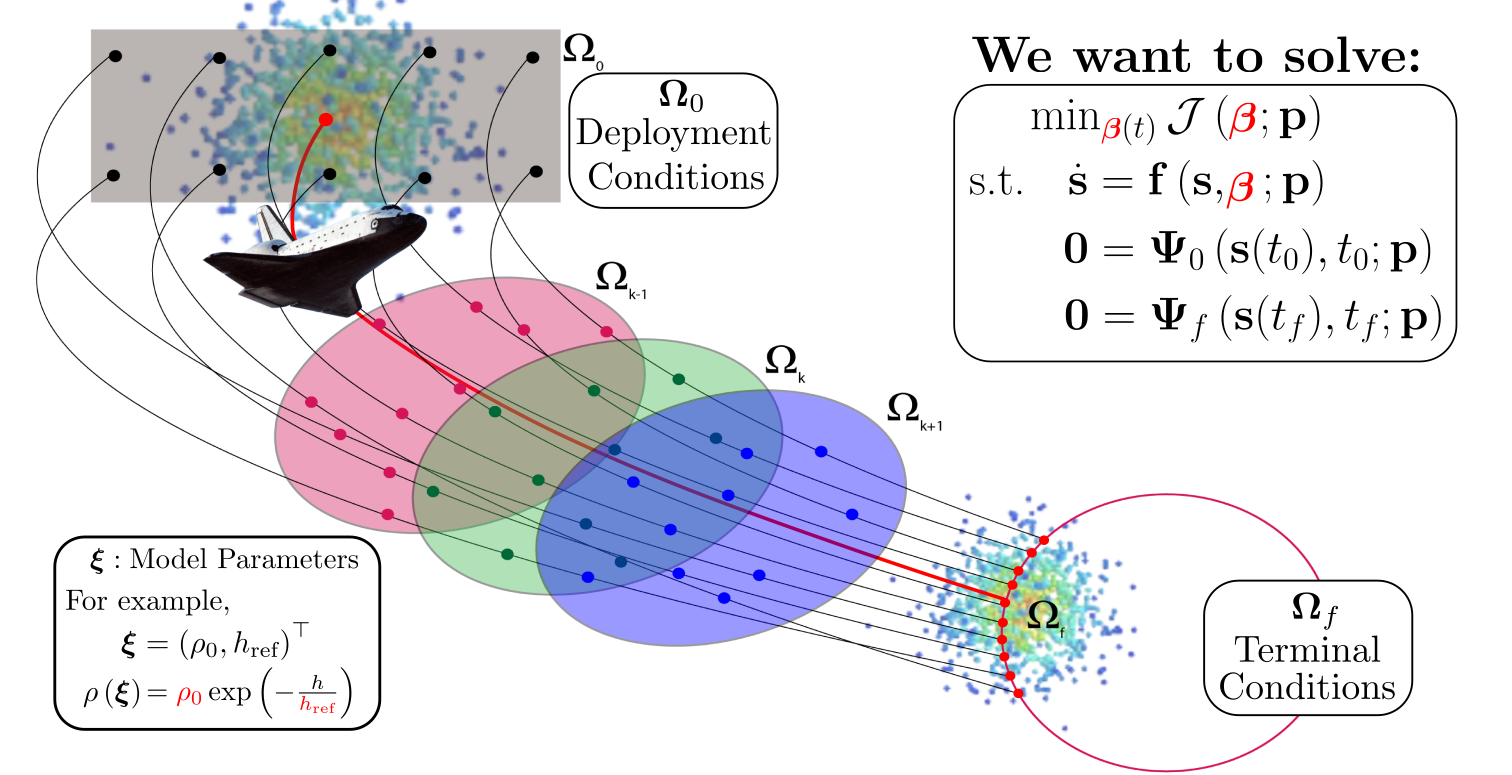
\includegraphics[width=0.9\textwidth]{../figs/sparsehjb/trajectory_parametrization_3.png}
            \end{figure}
        \end{column}
        \hspace*{-0.5in}
        \begin{column}{0.4\textwidth}
            \begin{graybox}{Parametrization}
                Parameters,
                \begin{equation*}
                    \vp = \left(\vOmega_0,\vOmega_f,\vxi\right)^\top\in\mathbb{R}^{n_p}
                \end{equation*}
                are, e.g., normally distributed,
                \begin{equation*}
                    \vp\sim\mathcal{N}\left(\mathbf{m},\boldsymbol{\sigma}\right)
                \end{equation*}
                where,
                \begin{itemize}
                    \item $\mathbf{m}$: nominal mission,
                    \item $\boldsymbol{\sigma}$: mission uncertainty
                \end{itemize}
            \end{graybox}
        \end{column}
    \end{columns}
\end{frame}

\begin{frame}{\small Generate a sparse high fidelity \textbf{distribution of optimal paths},}
    \footnotesize
    \begin{figure}
        \centering
        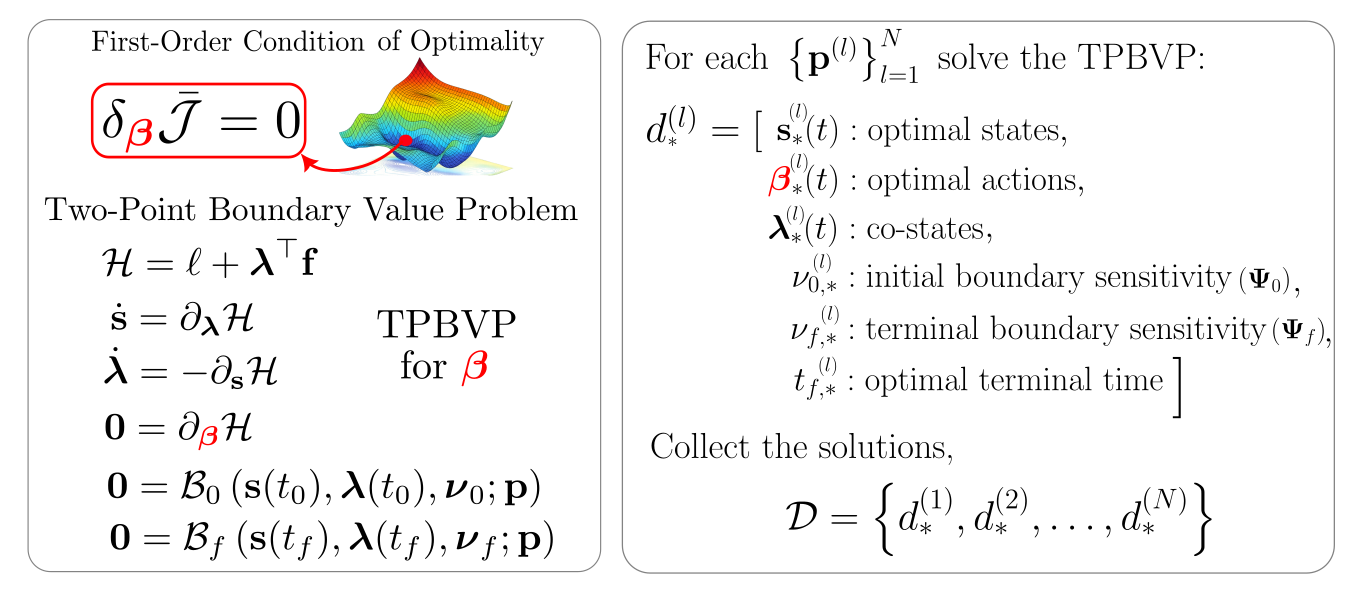
\includegraphics[width=0.9\textwidth]{../figs/sparsehjb/solutions_4.png}
    \end{figure}
\end{frame}

\begin{frame}{\small \textbf{Learn the value function} from the sparse high fidelity data,}
    \footnotesize
    \begin{figure}
        \centering
        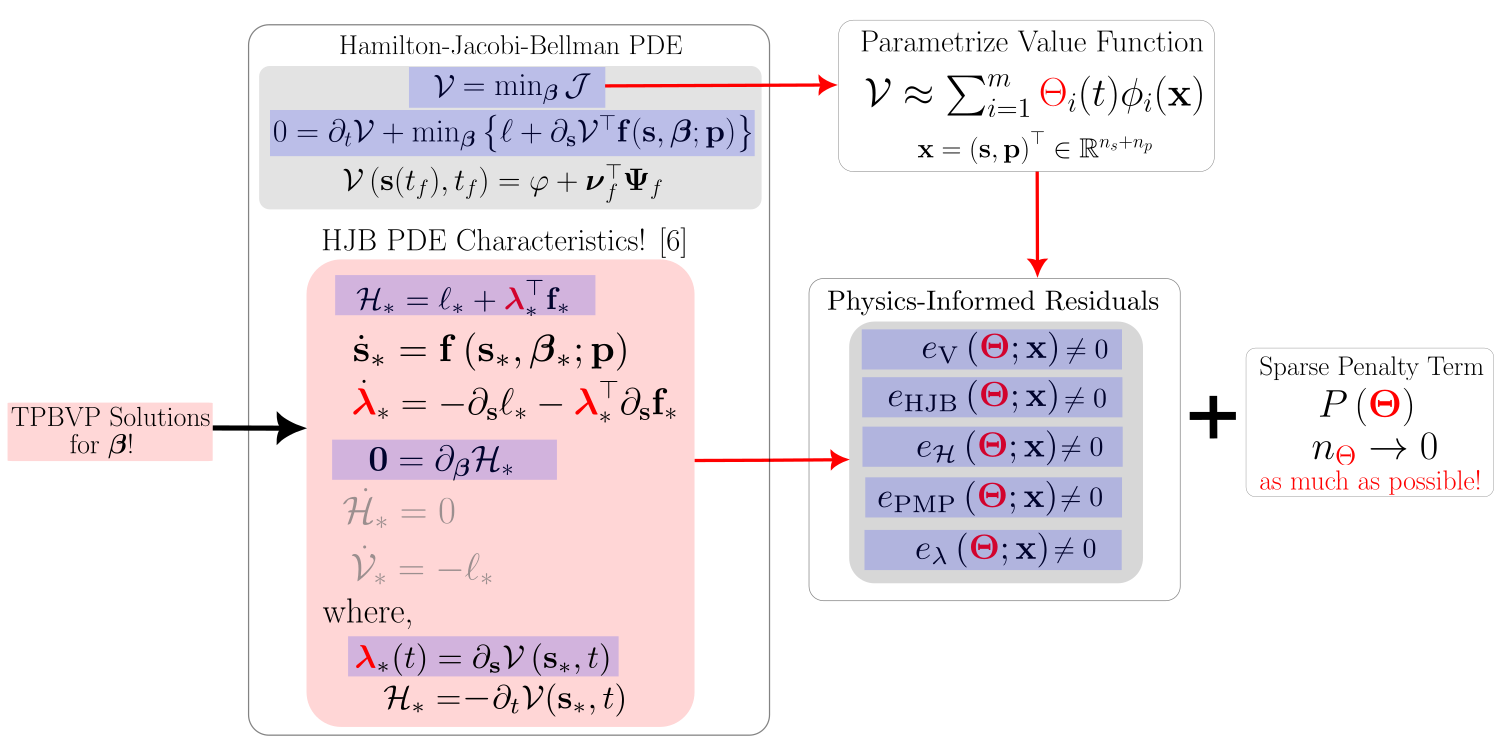
\includegraphics[width=0.95\textwidth]{../figs/sparsehjb/characteristics_12.png}
    \end{figure}
\end{frame}

\begin{frame}{\small We can \textbf{learn the value function} with controllable \textbf{efficiency and accuracy},}
    \footnotesize
    \begin{figure}
        \centering
        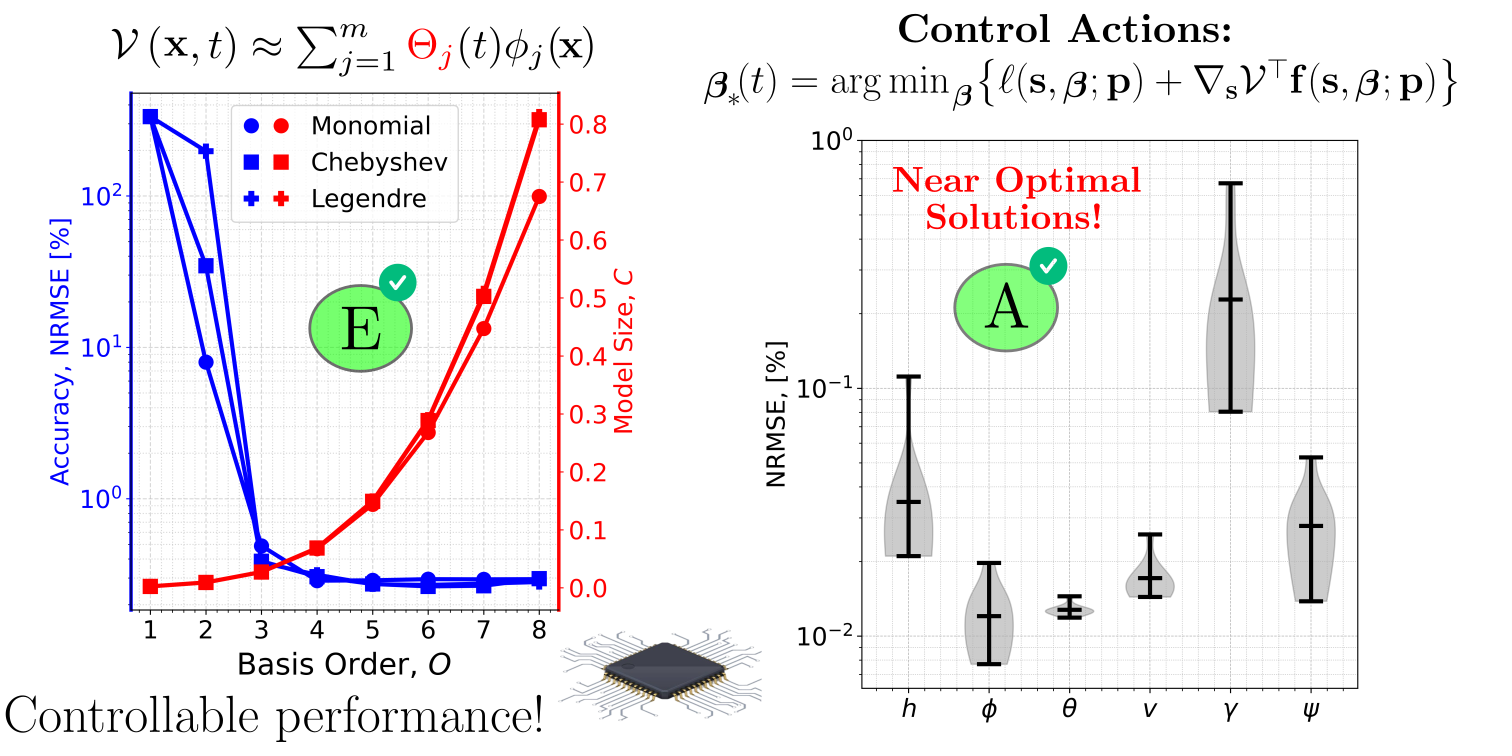
\includegraphics[width=0.9\textwidth]{../figs/sparsehjb/performance_ae_4.png}
    \end{figure}
\end{frame}

\begin{frame}{\small Real-time control for the \textbf{space shuttle during re-entry} to maximize \textbf{cross-range},}
    \footnotesize
    \begin{columns}
        \begin{column}{0.7\textwidth}
            \begin{figure}
                \centering
                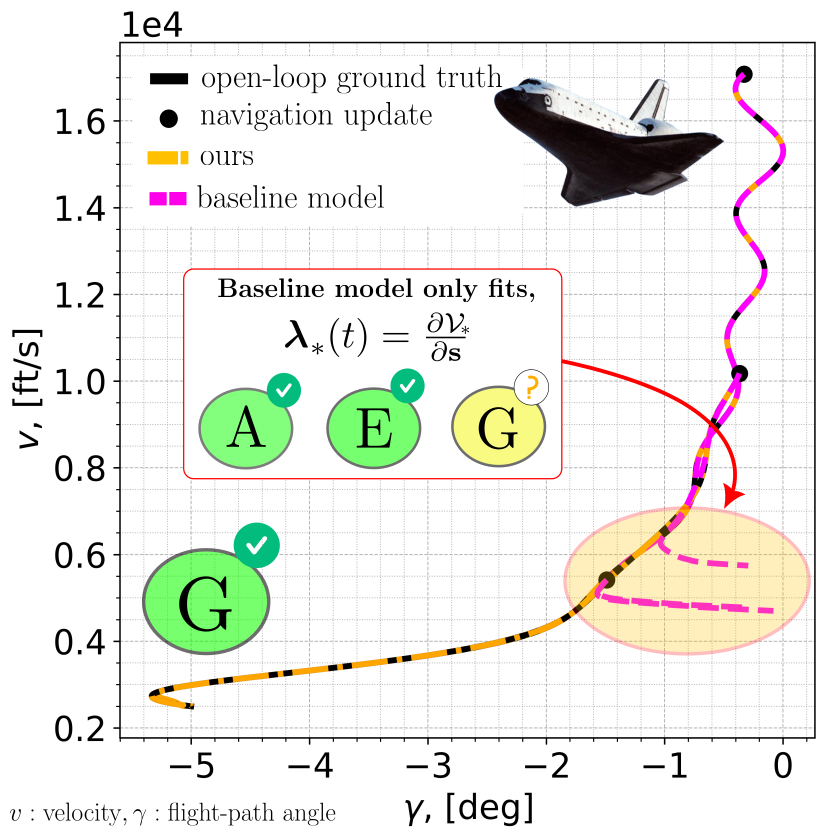
\includegraphics[width=0.65\textwidth]{../figs/sparsehjb/performance_ss_4.png}
            \end{figure}
        \end{column}
        \hspace*{-1in}
        \begin{column}{0.4\textwidth}
            \begin{graybox}{Key Results}
                \begin{itemize}
                    \item Improved \textbf{generalizability},
                    \item \textbf{Accelerations} $\approx10^4$,
                    \item \textbf{Model compressions} $\approx30\%$
                \end{itemize}
            \end{graybox}
        \end{column}
    \end{columns}
\end{frame}

\begin{frame}{\small Is the Impossible Trinity of Optimal Control \textbf{solved}?}
    \footnotesize
    \begin{columns}
        \begin{column}{0.4\textwidth}
            \centering
            \begin{figure}
                \centering
                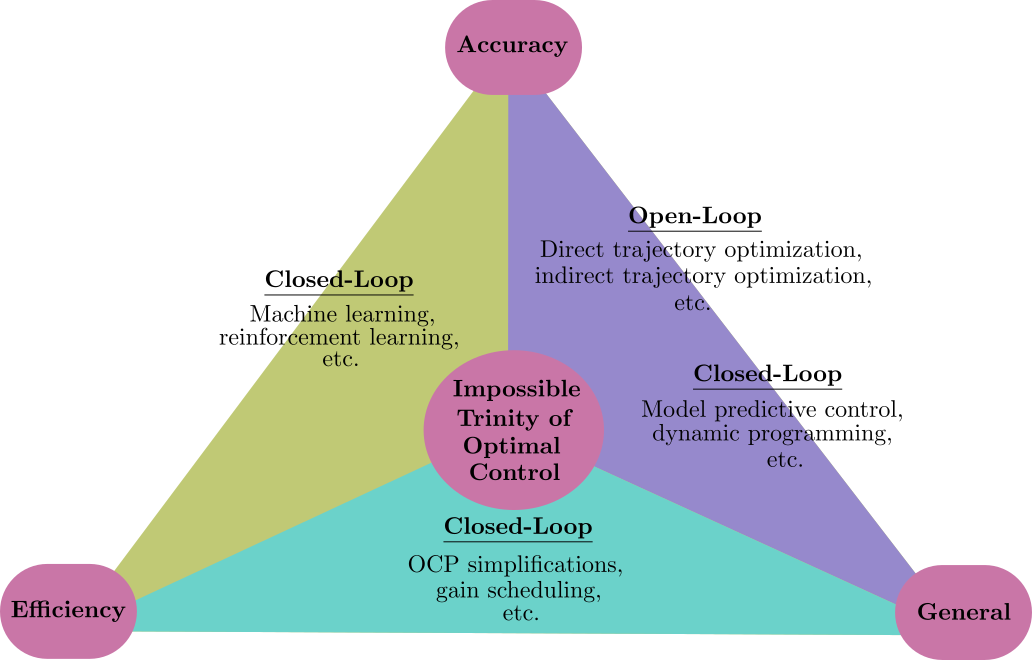
\includegraphics[width=0.9\textwidth]{../figs/introduction/itoc.png}
            \end{figure}
        \end{column}
        \begin{column}{0.7\textwidth}
            \centering
            \begin{itemize}
                \item \textbf{Accuracy}: comparable to indirect OCP solutions (NRMSE $<1\%$)
                \item \colorbox{green!30}{\textbf{Efficiency}}:
                \begin{itemize}
                    \item \colorbox{green!30}{\textbf{Accelerations} $\approx 10^3 - 10^4$}
                    \item \colorbox{green!30}{\textbf{Model compressions} $\approx 80\%$}
                \end{itemize}
                \item \colorbox{green!30}{\textbf{Generalizability}: unseen BCs and model parameters}, but no guarantees outside the tube!
                \item Offline training costs \colorbox{red!30}{not quantified (future work)}
            \end{itemize}
        \end{column}
    \end{columns}
    \begin{tikzpicture}[remember picture, overlay]
        \node[anchor=north west, xshift=2.2cm, yshift=-2.2cm] at (current page.north west) {
\includegraphics[width=0.1\textwidth]{../figs/pirom/checkmark.png}};
    \end{tikzpicture}
    \begin{tikzpicture}[remember picture, overlay]
        \node[anchor=north west, xshift=0.1cm, yshift=-5.1cm] at (current page.north west) {
\includegraphics[width=0.1\textwidth]{../figs/pirom/checkmark.png}};
    \end{tikzpicture}
    \begin{tikzpicture}[remember picture, overlay]
        \node[anchor=north west, xshift=4.45cm, yshift=-5.1cm] at (current page.north west) {
\includegraphics[width=0.1\textwidth]{../figs/pirom/checkmark.png}};
    \end{tikzpicture}
\end{frame}